\section{工厂生产计划设计(问题一)} % (fold)
\label{sec:工厂生产计划设计_问题一_}

\subsection{模型的建立} % (fold)
\label{sub:模型的建立}

% subsection 模型的建立 (end)
本题要求制定每周7天的生产计划,使总成本最小。
工厂生产成本可分为两个部分:
\begin{enumerate}
	\item 各部件生产的生产准备费用\\
只与组件相关,与开工时间无关、任一天开工的生产准备费均相等,后文记为$s^r$;
	\item 各部件的存贮费用\\
共有12种产品($R=12$),在每个时间阶段(本题将一周七天订为整个时间跨度$T$,并等分为七个时间阶段$t$)结尾,如果有产品$r$库存,则需支付相应的储存费用,单件产品1个时段的存贮费为$h^r$。
\end{enumerate}
另外,由于产品A、B、C的加工过程需占用关键设备,消耗的时间不可忽略,记为工时$c^r(r\in \text{\{A,B,C\}})$。

为了使总成本最小,本文以总成本$z$为目标函数,建立线性规划模型。
目标函数如下:

\begin{equation}
	\min z=\sum_{t=1}^{T} \sum_{r=1}^{R}\left(s^{r} \omega_{t}^{r}+h^{r} y_{t}^{r}\right).
\end{equation}
上式中,$h^{r} y_{t}^{r}$表示产品$r$库存的存贮费,其中,$y_{t}^{r}$是该产品的存贮数量;
$s^{r} \omega_{t}^{r}$表示部件$r$生产的生产准备费用,
这里的$\omega_{t}^{r}$是为了表述在$t$时段是否生产组件$r$, 从而确定是否要支付生产准备费, 而引用的0$\textendash$1变量
\begin{equation}
	\omega_{t}^{r}=\left\{\begin{array}{l}
1, \quad x_{t}^{r}>0 \\
0, \quad x_{t}^{r}=0
\end{array},\quad t=1,2, \cdots, T, r=1,2, \cdots, R.\right.
\end{equation}

题目中还要求生产周期开始时没有任何组件库存,周期结束后也不留下任何组件库存,且部件采购与WPCR组装没有延迟,故应满足以下约束条件:

\begin{itemize}
	\item 库存数量\\
	组件$r$在第$t$天的库存量,应为前一日的库存量$y_{t-1}^{r}$与当日组装数量$x_{t}^{r}$之和,再减去当日为生产组件$r'$而消耗的数量
	\begin{equation}
		y_{t}^{r}=y_{t-1}^{r}+x_{t}^{r}-\eta_{r^{\prime}}^{r} x_{t}^{r^{\prime}},\quad t=1,2, \cdots, T, r=1,2, \cdots, R.
	\end{equation}
	上式中,$\eta_{r^{\prime}}^{r}$为组装一个产品$r'$所需特定组件$r$的数量。

	\item WPCR需求量\\
	WPCR每日供应量应等于当日的WPCR外部需求数$d_t$
	\begin{equation}
		y_{t-1}^{\mathrm{WPCR}}+x_{t}^{\mathrm{WPCR}}-y_{t}^{\mathrm{WPCR}}=d_{t}, \quad t=1,2, \cdots, T
	\end{equation}

	\item 逻辑变量\\
	为了表示在$t$时段是否生产组件$r$,从而确定是否要支付生产准备费,引用0$\textendash$1变量$\omega_{t}^{r}$,等于1表示生产,反之表示不生产
	\begin{equation}\label{key1}
		\omega_{t}^{r}=\left\{\begin{array}{l}
		1, \quad x_{t}^{r}>0 \\
		0, \quad x_{t}^{r}=0
		\end{array},\quad t=1,2, \cdots, T, r=1,2, \cdots, R.\right.
	\end{equation}
	这里使用组件$r$的组装数量$x_{t}^{r}$是否大于0,来判断是否需要生产准备费。

	\item 生产总工时\\
	产品A、B、C的加工过程需占用关键设备,消耗的时间不可忽略,记为工时满足下式
	\begin{equation}\label{key2}
		\sum_{r=1}^{R} c^{r} x_{t}^{r} \leqslant M_{t},\quad t=1,2, \cdots, T,
	\end{equation}
	各部件生产工时之和应小于总生产工时。

	\item 题中所给边界条件\\
	要求生产周期开始时没有任何组件库存,周期结束后也不留下任何组件库存,因此,令:
	\begin{equation}\label{边界条件}
		y_{0}^{r}=y_{T}^{r}=0,\quad  r=1,2, \cdots, R.
	\end{equation}

	\item 非负约束\\
	显然,组件$r$(包括 WPCR)的组装数量与库存数量应为非负数
	\begin{equation}
		x_{t}^{r},  y_{t}^{r} \geqslant 0, \quad t=1,2, \cdots, T, r=1,2, \cdots, R.
	\end{equation}
\end{itemize}

	由于式\ref{key1}不便直接用程序计算,故将式\ref{key1}、\ref{key2}合并为下式\cite{姜启源2011数学模型}
	\begin{equation}
		\begin{array}{c}\label{修正式}
c^{r} x_{t}^{r}=M_{t}^{r} \omega_{t}^{r}, \quad t=1,2, \cdots, T, r=1,2, \cdots, R; \\
x_{t}^{r}=x_{t}^{r} \omega_{t}^{r},\quad t=1,2, \cdots, T, r=1,2, \cdots, R;\\
\sum_{r=1}^{R} M_{t}^{r} \leqslant M_{t}; \\
M_{t}^{r} \leqslant M_{t}^{r} \omega_{t}^{r}, \quad t=1,2, \cdots, T, r=1,2, \cdots, R;\\
M_{t}^{r} \geqslant 0,\quad  r=1,2, \cdots, R.
\end{array}
	\end{equation}
	不难发现,当$\omega_{t}^{r} = 0$时,$x_{t}^{r}$必然为0, 反之亦然,此次变换为编程实现提供了便利。


\subsection{模型的求解} % (fold)
\label{sub:模型的求解}

题中要求制定每周7天的生产计划,故有$T = 7$。综上,建立的线性规划模型如下:
\begin{equation}\label{总模型}
	\begin{aligned}
&\min \quad z  = \sum_{t  = 1}^{T} \sum_{r = 1}^{R}\left(s^{r} \omega_{t}^{r}+h^{r} y_{t}^{r}\right)\\
& \ \begin{array}{r@{\quad}l@{}l@{\quad}l}
\mathrm{s.t. } 	&\sum_{r=1}^{R} M_{t}^{r} \leqslant M_{t}; &\\
&M_{t}^{r} \leqslant M_{t}^{r} \omega_{t}^{r}, &t=1,2, \cdots, T, r=1,2, \cdots, R;\\
& y_{t}^{r}=y_{t-1}^{r}+x_{t}^{r}-\eta_{r}^{r} x_{t}^{r^{\prime}}, &t=1,2, \cdots, T,  r=1,2, \cdots, R; \\
&\omega_{t}^{r} \in\{0,1\}, &t=1,2, \cdots, T, r=1,2, \cdots, R; \\
&x_{t}^{r}=x_{t}^{r} \omega_{t}^{r},& t=1,2, \cdots, T, r=1,2, \cdots, R;\\
&c^{r} x_{t}^{r}=M_{t}^{r} \omega_{t}^{r}, &t=1,2, \cdots, T, r=1,2, \cdots, R; \\
&M_{t}^{r} \geqslant 0,& r=1,2, \cdots, R ;\\
&y_{0}^{r}=y_{T}^{r}=0,& r=1,2, \cdots, R ;\\
&x_{t}^{r}, y_{t}^{r} \geqslant 0, &t=1,2, \cdots, T, r=1,2, \cdots, R;\\
&y_{t-1}^{\mathrm{WPCR}}+x_{t}^{\mathrm{WPCR}}-y_{t}^{\mathrm{WPCR}}=d_{t}, & t=1,2, \cdots, T; \\
\end{array}.
\end{aligned}
\end{equation}



从一方面来说,本模型同时包含连续变量和整数变量,是混合整数规划。
从另一方面, 由于目标函数和约束条件对于决策变量而言都是线性的,所以本模型为线性规划。
因此,本模型为混合线性规划模型,存在最优解且已有许多可靠的求解器以供使用。

\subsection{生产方案展示} % (fold)
\label{sub:生产方案展示}

\begin{table}
\centering
\caption{问题一的结果}
\resizebox{\linewidth}{!}{
\begin{tabular}{ccccccccccccccc}
\toprule
\diagbox{日期}{部件(花费)} & WPCR & B    & A   & C    & B2   & B1   & A2   & A3   & A1   & C1    & C2   & C3    & 生产准备费用 & 生产库存费用              \\
\midrule
周一                   & 83   & 332  & 249 & 416  & 1328 & 664  & 1992 & 498  & 1494 & 3328  & 832  & 4992  & 1200   & 221.7               \\
周二                   & 0    & 344  & 0   & 0    & 1376 & 688  & 0    & 0    & 0    & 0     & 0    & 0     & 340    & 557.7               \\
周三                   & 81   & 0    & 243 & 404  & 0    & 0    & 1944 & 486  & 1458 & 3232  & 808  & 4848  & 860    & 285                 \\
周四                   & 0    & 0    & 0   & 0    & 0    & 0    & 0    & 0    & 0    & 0     & 0    & 0     & 0      & 85                  \\
周五                   & 48   & 173  & 144 & 240  & 692  & 346  & 1152 & 288  & 864  & 1920  & 480  & 2880  & 1200   & 111.5               \\
周六                   & 51   & 203  & 153 & 255  & 812  & 406  & 1224 & 306  & 918  & 2040  & 510  & 3060  & 1200   & 200                 \\
周天                   & 0    & 0    & 0   & 0    & 0    & 0    & 0    & 0    & 0    & 0     & 0    & 0     & 0      & 0              \\
\cline{14-15}
总和                   & 263  & 1052 & 789 & 1315 & 4208 & 2104 & 6312 & 1578 & 4734 & 10520 & 2630 & 15780 & \multicolumn{2}{c}{6260.9}  \\
\bottomrule
\end{tabular}
}
\end{table}

一般地,工厂为降低总成本有两种策略,分别是:开车型和仓储型。
极端地,选择开车型的工厂将每个时段均进行生产以满足且仅满足所在时段需求,来尽可能减少库存费;而选择仓储型的工厂会把生产任务集中安排,来尽可能减少生产准备费,代价是会损失因产品积压导致的库存费。
然而,由于关键设备总工时的限制,这两种策略不一定能不折不扣地实施(如:实际计算发现,周日的需求不能仅靠当日生产满足、也不存在任何一天能组装出满足一周需求的产品)。
故模型的最优解正是这两种策略达到平衡时的状态。

\begin{figure}[!htbp]
	\centering
	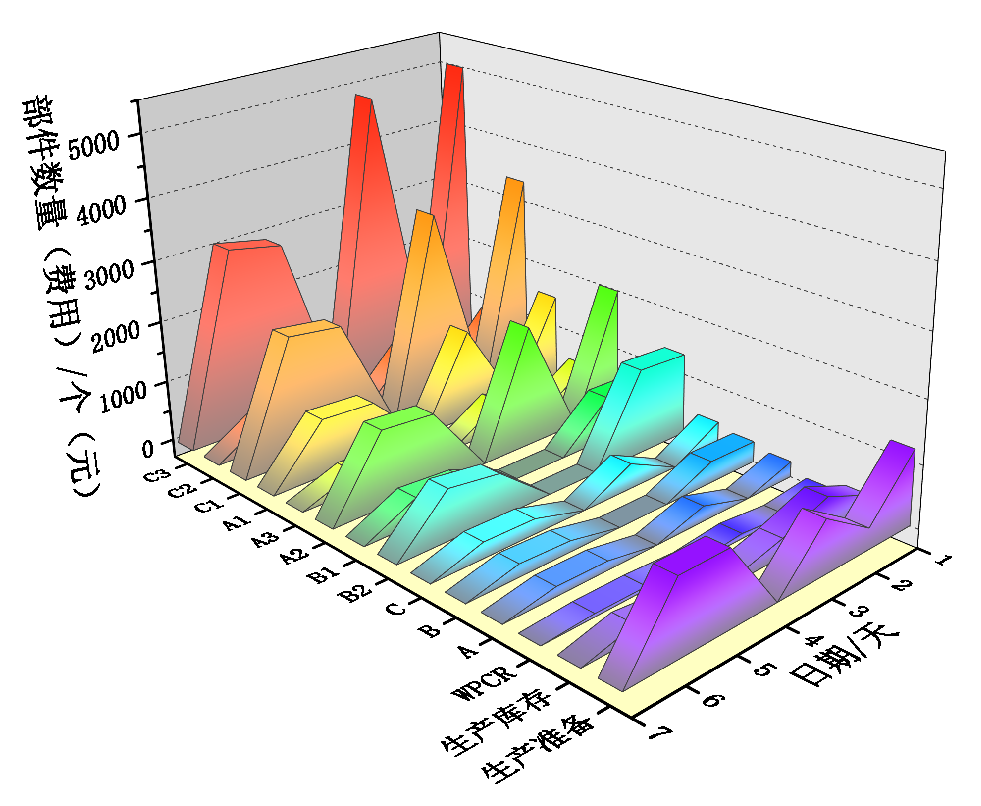
\includegraphics{Image/问题一展示.eps}
	\caption{各组件的当日组装数量及生产费用}\label{各组件的当日组装数量及生产费用}
\end{figure}


\begin{figure}[!htbp]
	\centering
	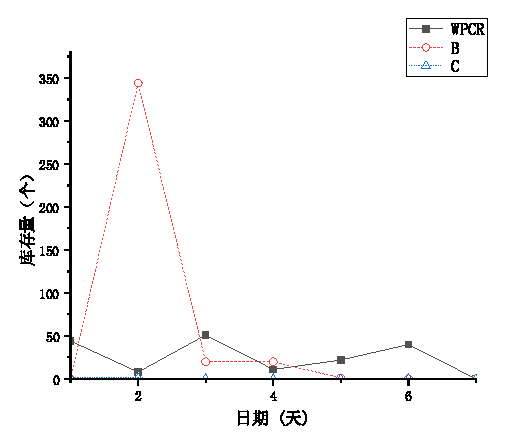
\includegraphics{Image/问题一库存.eps}
	\caption{每日组件库存数量变化}\label{每日组件库存数量变化}
\end{figure}

图2中未绘出的组件库存数量始终为0,有效节省了大量库存费用;结合图1可知该工厂频繁开车,本文认为该工厂总体上选择了开车型策略.
这是不难理解的——其余三个问题中,库存费用远高于生产准备费、是节约成本的主要矛盾,因此工厂选用开车型策略来最小化库存费用是合理的.

然而,仓储型策略也在一定程度上参与了工厂生产的计划,周四和周日显著体现了仓储型工厂的决策特点.
周四和周日的生产总工时限制最严、但WPCR需求又最大,这提示生产总工时限制对决策产生的影响比WPCR需求大.

% subsection 生产方案展示 (end)

% subsection 模型的求解 (end)





% section 工厂生产计划设计_问题一_ (end)
